\chapter{The JUNO experiment}

The first idea of a medium baseline (~60 km) experiment, was explored in 2008 where it was demonstrated that the Neutrino Mass Ordering (NMO) could be determined by a medium baseline experiment if $\sin^2(2\theta_{13}) > 0.005$ without requirements on accurate information of the reactor antineutrino spectra and the value of $\Delta m_{32}^2$. \cite{zhan_determination_2008}. From this idea is born the Jiangmen Underground Neutrino Observatory (JUNO) experiment.

JUNO is a neutrino detection experiment under construction located in China. Its main objective is the determination of the mass ordering at the 3-4$\sigma$ level in 6 years of data taking and the measurement at the per-mil precision of the oscillation parameters $\Delta m_{21}^2$, $\sin^2 2\theta_{12}$, $\Delta m_{32}^2$ and, with less precision, $\sin^2\theta_{13}$\cite{an_neutrino_2016}.

\section{Neutrinos physics in JUNO}

While the design of JUNO is tailored to measure $\bar{\nu_e}$ coming from nuclear reactor, JUNO will be able to detect neutrinos coming from other sources thus allowing for a wide range of physics studies as detailed in the table \ref{tab:signal} and in the following sub-section.

\begin{table}
\begin{center}
  \begin{tabular}{|c|c|c|c|}
    \hline Research & Expected signal & Energy region & Major backgrounds \\
    \hline Reactor antineutrino & 60 IBDs/day & 0–12 MeV  & Radioactivity, cosmic muon \\
    Supernova burst & 5000 IBDs at 10 kpc & 0–80 MeV & Negligible \\
                    & 2300 elastic scattering  & &  \\
    DSNB (w/o PSD) & 2–4 IBDs/year & 10–40 MeV & Atmospheric $\nu$ \\
    Solar neutrino & hundreds per year for $^8$B & 0–16 MeV & Radioactivity \\
    Atmospheric neutrino & hundreds per year & 0.1–100 GeV  & Negligible \\
    Geoneutrino &  $\approx 400$ per year & 0–3 MeV & Reactor $\nu$ \\
    \hline
  \end{tabular}
  \caption{Detectable neutrino signal in JUNO and the expected signal rates and major background sources}
  \label{tab:signal}
\end{center}
\end{table}

\subsection{Reactor neutrino oscillation for NMO and precise measurements}

Previous works \cite{zhan_determination_2008,  zhan_experimental_2009} shows that oscillation parameters and the NMO can be observed by looking at the $\bnue$ disappearance spectrum coming from medium baseline nuclear reactor. This disappearance probability can be expressed as \cite{an_neutrino_2016} :
\begin{equation*}
  P(\bnue \rightarrow \bnue) = 1 - \sin^2 2\theta_{12} c^4_{13} sin^2 \frac{\Delta m^2_{21}L}{4E} - \sin^2 2\theta_{13} \bigg[ c_{12}^2 \sin^2 \frac{\Delta m_{31}^2 L}{4E} + s^2_{12} \sin^2 \frac{\Delta m_{32}^2 L}{4E} \bigg]
\end{equation*}
Where $s_{ij} = \sin \theta_{ij}$, $c_{ij} = \cos \theta_{ij}$, $E$ is the $\bnue$ energy and $L$ is the baseline.
We can see the sensitivity to the NMO in the dependency to $\Delta m_{32}^2$ and $\Delta m^2_{31}$ causing a phase shift of the spectrum as we can see in the figure \ref{fig:juno-spectrum-oscillation}.
By carefully fitting this spectrum, one can extract the NMO and the oscillation parameters.

\begin{figure}
  \centering
  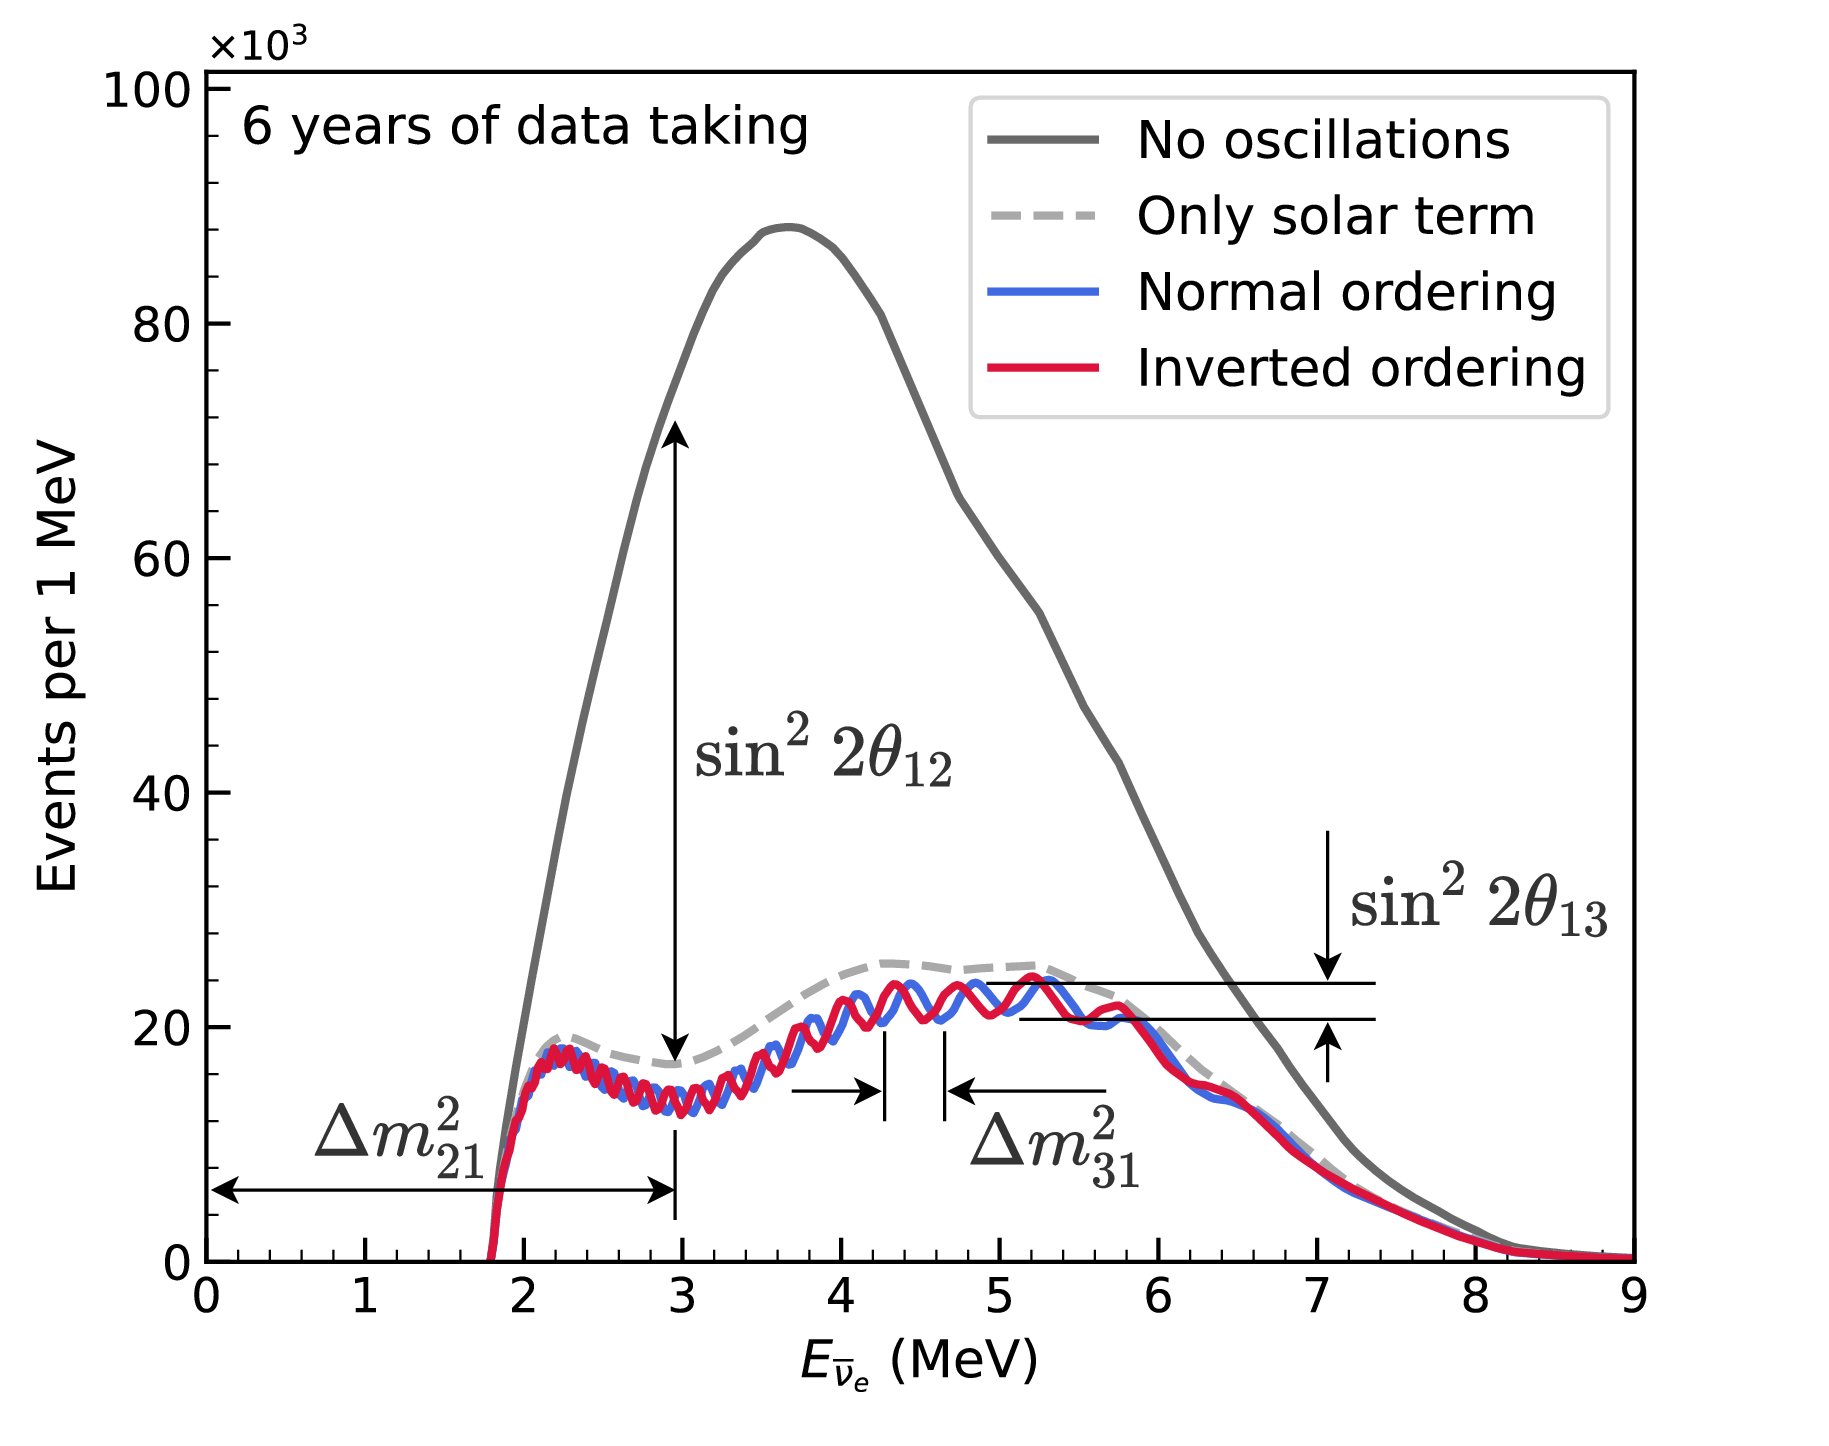
\includegraphics[height=8cm]{images/juno/Spectrum-OscillationsOnly_dm2_31.png}
  \caption{Expected number of neutrinos event per MeV in JUNO after 6 years of data taking. The black curve shows the flux if there was no oscillation. The light gray curve shows the oscillation if only the solar terms are taken in account ($\theta_{12}$, $\Delta m_{21}^2$). The blue and red curve shows the spectrum in the case of, respectively, NO and IO. The dependency of the oscillation to the different parameters are schematized by the double sided arrows. We can see the NMO sensitivity by looking at the fine phase shift between the red and the blue curve.}
  \label{fig:juno-spectrum-oscillation}
\end{figure}

To reach the desired sensitivity, JUNO must meet multiple requirements but most notably:
\begin{enumerate}
  \item An energy resolution of $3\%/\sqrt{E\mathrm{(MeV)}}$ to be able to distinguish the fine structure of the fast oscillation.
  \item An energy precision of 1\% in order to not err on the location of the oscillation pattern.
  \item A baseline of 53 $\pm$ 0.5 km to maximise the $\bar{\nu_e}$ oscillation probability.
  \item At least $\approx$ 100,000 events to limit the spectrum distortion dur to statistical uncertainties.
\end{enumerate}

\subsubsection{Identification of the mass ordering}

To identify the mass ordering, we fit the neutrino energy spectrum under the two hypothesis of NO and IO. Those two fit give us two $\chi^2$, respectively $\chi^2_{NO}$ and $\chi^2_{IO}$. By computing the difference $\Delta \chi ^2 = \chi^2_{NO} - \chi^2_{IO}$ we can determine the most probable mass ordering: NO if $\Delta \chi^2 > 0$ and IO if $\Delta \chi^2 < 0$. Current studies shows that the expected sensitivity the mass ordering would be of $3.4 \sigma$ after 6 years of data taking in nominal setup\cite{an_neutrino_2016}.

\subsubsection{Precise measurement of the oscillations parameters}

The oscillations parameters $\theta_{12}$, $\theta_{13}$, $\Delta m^2_{21}$, $\Delta m^2_{31}$ are free parameters in the fit of the oscillation spectrum. The precision on those parameters have been estimated and are shown in figure \ref{fig:juno-param-precision}. Wee see that for $\theta_{12}$, $\Delta m^2_{21}$, $\Delta m^2_{31}$, precision at 6 years is better than the reference precision by an order of magnitude \cite{juno_collaboration_sub-percent_2022}

\begin{figure}[hb]
  \centering
  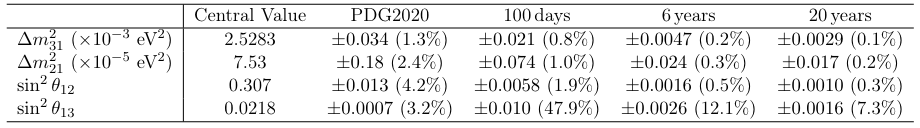
\includegraphics[width=\linewidth]{images/juno/oscillation_params_precision.png}
  \caption{A summary of precision levels fir the oscillation parameters. The reference value (PDG 2020 \cite{pdg2020}) is compared with 100 days, 6 years and 20 years of JUNO data taking.}
  \label{fig:juno-param-precision}
\end{figure}

\subsection{Other physics}

While reactor neutrinos are the main signal, JUNO will of course be sensitive to every neutrinos energetic enough to allow an IBD, and even some other more exotic channels.

\subsubsection{Geoneutrinos}

Geoneutrinos designate the antineutrinos coming from the decay of long-lived radioactive elements inside the Earth. The 1.8 MeV threshold necessary for the IBD makes it possible to measure geoneutrinos from $^238$U and $^232$Th decay chains. The studies of geoneutrinos can help refine the Earth crust models but is also necessary to characterise their signal, as they are a background to the mass ordering and oscillations parameters studies.

\subsubsection{Atmospheric neutrinos}

Atmospheric neutrinos are neutrinos originating from the decay of $\pi$ and $K$ particles that are produced in extensive air showers initiated by the interactions of cosmic rays with the Earth atmosphere. Earth is mostly transparent to neutrinos below the PeV energy, thus JUNO will be able to see neutrinos coming from all directions. Their baseline range is large (15km $\sim$ 13000km), they can have energy between 0.1 GeV and 10 TeV and will contain all neutrino and antineutrinos flavour. Their studies is complementary to the reactor antineutrinos and can bring constraint on the MO \cite{an_neutrino_2016}.

\subsubsection{Beyond standard model neutrinos interactions}

JUNO will also be able to probe for beyond standard model neutrinos interactions. After that the main physics topics have been accomplished, JUNO could be upgraded to probe for neutrinoless beta decay ($0\nu\beta\beta$). The detection of such event would give critical informations about the nature of neutrinos, is it a majorana or a dirac particle. JUNO will also be able to probe for neutrinos that would come for the decay or annihilation of Dark Matter inside the sun and neutrinos from putative primordial black hole.
Through the unitary test of the mixing matrix, JUNO will be able to search for light sterile neutrinos.
Thanks to JUNO sensitivity, multiple other exotic can be performed on neutrino related beyond standard model interactions.

\subsubsection{Supernovae burst neutrinos}

Neutrinos are crucial component during all stages of stellar collapse and explosion. Detection of neutrinos coming for core collapse supernovae will provide us important informations on the mechanisms at play in those events.
Thanks to its 20 kt LS, JUNO has excellent capabilities to detect all flavour of the $\mathcal{O}$(10 MeV) postshock neutrinos, and using neutrinos of the $\mathcal{O}$(1 MeV) will give informations about the pre-supernovae neutrinos. All those informations will allow to disentangle between the multiple hydro-dynamic models that are currently used to describe the different stage of the core-collapse.

\subsubsection{Diffuse supernovae neutrinos background}

Core-collapse supernovae in our galaxy are rare events, but they frequently occur throughout the visible Universe sending burst of neutrinos in direction of the Earth. All those events contributes to a low background flux of low-energy neutrinos called the Diffuse Supernovae Neutrino Background (DSNB). Its flux and spectrum contains informations about the red-shift dependent supernovae rate, the average SN neutrino energy and the fraction of black-hole formation in core-collapse supernovae. Depending of the DSNB model, we can expect 2-4 IBD events per year in the energy range above the reactor $\bar{\nu_e}$ signal, which is competitive with the current Super-Kamiokande+Gadolinium phase.

\subsubsection{Background in the neutrinos reactor spectrum}



\section{The JUNO detector}

\subsection{Central Detector (CD)}

\subsubsection{Acrylic containment sphere}

\subsubsection{Liquid scintillator}

\subsubsection{Large photo-multipliers (LPMTs)}

\subsubsection{Small photo-multipliers (SPMTs)}

\subsubsection{Data Acquisition System (DAQ)}

\subsubsection{Simulation}

\subsubsection{Software}

\todo{Expliquer comment le software fonctionne}


\subsection{Veto detector}

\subsubsection{Cherenkov in water pool}

\subsubsection{Top tracker}

\section{Calibration strategy}

\subsection{Energy scale calibration}

\subsection{Calibration system}

\subsection{Calibration program}

\section{Event selection and background rejection}

\todo{Explication de comment reconnaitre un IDB (OEC)}

\subsection{Fiducial volume}

\subsection{Muon tagging}

\section{State of the art of the IBD reconstruction}

\subsection{Interaction vertex reconstruction}

\subsection{Energy reconstruction}

\subsection{Particle identification}

\subsection{Machine learning for reconstruction}

\subsubsection{Vertex reconstruction}

\subsubsection{Energy reconstruction}

\section{JUNO sensitivity to NMO and precise measurements}

\subsection{Fitting procedure}
